\documentclass[12pt]{article}
\usepackage{enumerate, amsmath, fullpage, hyperref, amsfonts, titlesec, listings, graphicx, enumitem, longtable, tikz}
\usetikzlibrary{calc,trees,positioning,arrows,chains,shapes.geometric,
    decorations.pathreplacing,decorations.pathmorphing,shapes,
    matrix,shapes.symbols}
\renewcommand*\contentsname{Table of Contents}
\newlength\tindent
\setlength{\tindent}{\parindent}
\setlength{\parindent}{0pt}
\renewcommand{\indent}{\hspace*{\tindent}}
\lstset{
   breaklines=true,
   basicstyle=\scriptsize\rmfamily}
\tikzset{
>=stealth',
  chain/.style={
    rectangle, 
    rounded corners, 
    % fill=black!10,
    draw=black, very thick,
    text width=10em, 
    minimum height=3em, 
    text centered, 
    on chain},
  line/.style={draw, thick, <-},
  element/.style={
    tape,
    top color=white,
    bottom color=blue!50!black!60!,
    minimum width=8em,
    draw=blue!40!black!90, very thick,
    text width=10em, 
    minimum height=3.5em, 
    text centered, 
    on chain},
  every join/.style={->, thick,shorten >=1pt},
  decoration={brace},
  tuborg/.style={decorate},
  tubnode/.style={midway, right=2pt},
}
\begin{document}
\thispagestyle{empty}
\begin{center}
  {\bf\Large Train Control Demo 2 / Final Train Demo}\\
  {\bf\large CS452 - Spring 2014}\\
  Real-Time Programming\vspace{5cm}\\
  {\bf Team }\\
  Max Chen - mqchen\\
  mqchen@uwaterloo.ca\\[1\baselineskip]
  Ford Peprah - hkpeprah\\
  ford.peprah@uwaterloo.ca\vspace{5cm}\\
  Bill Cowan\\
  University of Waterloo\\
\end{center}
\newpage
% Program Description: how to operate it, full pathname
% Description fo structure of Kernel: algorithms, data structures, etc.
% Location fo source code + MD5
% Output produced by program and explanation of why it does
\thispagestyle{empty}
\tableofcontents
\newpage
\section{Program Description}
\subsection{Getting the Program}
To run the program, one must have read/write access to the source code, as well as the ability to make and run the program.  Before attempting to run the pogram ensure that the following three conditions are met:
\begin{itemize}
  \item You are currently logged in as one of \texttt{cs452}, \texttt{mqchen}, or \texttt{hkpeprah}.
  \item You have a directory in which to store the source code, \\ e.g. \texttt{\textasciitilde/cs452\_microkern\_mqchen\_hkpeprah}.
  \item You have a folder on the FTP server with your username, e.g. \texttt{/u/cs452/tftp/ARM/cs452}.
\end{itemize}
First, you must get a copy of the code.  To to this, log into one of the aforementioned accounts and change directories to the directory you created above (using \texttt{cd}), then run one of
\begin{center}
  \begin{verbatim}
    git clone file:////u8/hkpeprah/cs452-microkern -b final .
                           or
    git clone file:////u7/mqchen/cs452/cs452-microkern -b final .
  \end{verbatim}
\end{center}
\vspace{-0.5cm}You will now have a working instance of our TC2/Final source code in your current directory.  To make the application and upload it to the FTP server at the location listed above (\texttt{/u/cs452/tftp/ARM/YOUR\_USERNAME}), run \texttt{make upload}.  This will generate our source code that is functional on Track A, since distances are different on both tracks, you should run by specifying the track you want to use.  To do so, you can use any of the options listed below to customize your generated ELF file:
\begin{center}
  {\bf Make Options} - Can only specify one
  \begin{tabular}{|l|c|c|}
    \hline
    {\bf Option} & {\bf Description} \\\hline
    upload & Make and upload the generated file. \\\hline
    debug & Make and upload the generated file with debugging enabled. \\\hline
    test & Make for testing. \\\hline
  \end{tabular}
\end{center}
\begin{center}
  {\bf Make Flags} - Multiple can be specified
  \begin{tabular}{|l|c|c|}
    \hline
    {\bf Flag} & {\bf Description} \\\hline
    \texttt{TRACK=a} or \texttt{TRACK=b} & Makes for track A or track B depending on specified. \\\hline
    \texttt{SILENT} & Make with debugging off for tests. \\\hline
    \texttt{PROFILING} & Make for testing profiling. \\\hline
    \texttt{TEST=filename.c} & Make a test file using the specified file as the main. \\\hline
    \texttt{TARGET=filename} & Make the code and store it in the specified elf file. \\\hline
  \end{tabular}
\end{center}
\\[1\baselineskip]
\subsection{Running the Program}
To run the application, you need to load it into the RedBoot terminal.  Ensure you've followed the steps listed above in the ``Getting the Program'' settings to ensure you have the correct directories and account set up.  Navigate to the directory in which you cloned the source code and run \texttt{make upload}.  The uploaded code should now be located at (depending on the track you made for, defaults to 'a'):
\begin{center}
  \texttt{/u/cs452/tftp/ARM/YOUR\_USERNAME/kernel-a.elf} \\
  \texttt{/u/cs452/tftp/ARM/YOUR\_USERNAME/kernel-b.elf}
\end{center}
To run the application, go to the RedBoot terminal and run the command
\begin{center}
  \texttt{load -b 0x00218000 -h 10.15.167.4 ``ARM/YOUR\_USERNAME/kernel.elf''; go}
\end{center}
The application should now begin by running through the game tasks before reaching a prompt.  The generated files will be located in \texttt{DIR/build} where \texttt{DIR} is the directory you created in the earlier steps.  To access and download an existing version of the code, those can be found at \texttt{/u/cs452/tftp/ARM/mqchen/kernel.elf} and \texttt{/u/cs452/tftp/ARM/hkpeprah/kernel.elf}.
\\
\subsubsection{Command Prompt}
After the startup tasks have finished running, the user will reach a command prompt where they will be able to enter commands.  A list of available commands and the syntax can be found at run-time by entering either ``?'' or ``help'' followed by the ``RETURN'' key.  All commands must be followed by the ``RETURN'' key for the {\tt Shell} to interpret them.
\\[2\baselineskip]
\section{Task Structure}
\\[2\baselineskip]
\section{Train Control Demo 2}
For the purpose of routing our trains from its current location to any provided location, we use a layered architecture
in which each feature is built and abstracted such that more advanced navigation systems can be created on top of them
without worrying about how they work. We provide an extremely simple interface (include/train\_task.h) to an extremely
complicated task (src/train/train\_task.c).

\subsection{Basic Train Driving}
The most basic functionality of the train is to just drive and know where it is (required for Demo 1). We accomplish
this by having each \texttt{TrainTask} create a slave task that sends into it every 5 ticks telling it to update its
location, as well as a hard resync with the track whenever our train hits a sensor. The train tracks a huge amount of
information, see Appendix A for details.
\\
Internal to the \texttt{TrainTask}, these are provided by the functions \texttt{setTrainSpeed} (change speed) and
\texttt{trainDir} (reverse). These are exposed as functions (wrappers for Send to the \texttt{TrainTask})
\texttt{TrSpeed} and \texttt{TrDir} respectively.

\subsection{Path Finding}
Path finding is implemented over the provided track graph using the heap version of Dijkstra's, taking into account
track reservation as well. If any node is reserved by another train, then the pathfinding algorithm will no longer use
that node. For each node, the algorithm will add its reverse, its straight edge, and in the case of branches, its curved
edge. The function \texttt{findPath} will fill the provided \texttt{track\_node*} array with nodes of the path, return
the number of nodes and write the total length of the path in mm in an output parameter.

\subsection{Reservation}
The reservation system was built into the provided \texttt{track\_node} graph by simply adding a field in the
\texttt{track\_node} struct called \texttt{reservedBy} that indicates the train number of the train that has the
particular node reserved. This could have been done in a more encapsulated way that hides this reservation as the
current method allows anyone with a \texttt{track\_node*} to modify the value. However, we decided to take the simpler
approach as time was limited, and trust that our two programmers will not modify the value directly, and instead use the
provided interfaces.
\\
At the heart of the reservation system is a compare-and-swap (CAS) function that isn't absolutely true to its name. The
function does the simple operation of comparing the existing reservedBy field to a provided value, and if they match,
sets it to the new value (more of a test-and-set). The operation is also idempotent, so when a train tries to reserve a
node it already owns the operation will succeed even though the comparison failed. The train number -1 is defined / used as
RESERVED\_BY\_NOBODY to indicate that a node is free. As such, a reserve and release simply call CAS for each provided
\texttt{track\_node*} from nobody to the train or the train to nobody, respectively.
\\
When a train needs to reserve more track, it should not modify \texttt{reservedBy}. Instead, it calls into a server,
the \texttt{Dispatcher}), so that modifications to the field are mutually exclusive. The functions (as always, wrappers
for a Send into the task) provide a train number and an array of \texttt{track\_node*}, and optionally a distance. The 
reservation system will then attempt to reserve track, following the array until it is exhausted. If a distance is
provided, then the system will reserve at most the provided distance, no more and no less. That is, if the provided path
array is longer than the distance, only the distance will be reserved. Conversely, if the provided path is not long
enough for the distance, then the reservation system will look ahead in the track graph and reserve until the provided
distance is met (one minor problem with this is that since we only have \texttt{track\_node} granularity, we are prone
to over-reserving a large portion of the track when we reach an extremely long edge).
\\
The reservation code will return the number of \texttt{track\_node} successfully reserved, as well as modify the
provided distance field (passed in as a pointer) such that it becomes the amount of distance that was not reserved.

\subsection{Collision Avoidance}
When a train asks for more track, it always provides a distance which is slightly greater than its stopping distance by
some factor. This ensure that the train will be able to stop in the amount of track it has reserved. If the stopping
distance field is ever positive (that is, the reservation system could not reserve all the provided distance) then the
train knows that it is approaching track reserved by another train, and will stop itself. Otherwise, the train obtains a
value that indicates how much extra distance it has before it must reserve more track. Once that extra distance runs
out, it will attempt to reserve track again.

\subsection{Basic Path Execution}
Basic path execution is done solely within the train, and does not support paths that include reversals. The function
\texttt{TrGotoAfter} is provided by the train that will drive the train, in a linear fashion, to some offset after the
provided \texttt{track\_node}. This is accomplished by recomputing the path length on every train state update and then
issuing the train speed command when the stopping distance is equal to the remaining path length.
\\
Path execution is done every time new nodes are reserved. When a node is reserved and the previous node is a switch,
then the switch is flipped to the state such that moving over the switch will lead us to the correct next node.

\subsection{Short Moves}
Short moves are accomplished by setting the train to a speed, waiting for some number of ticks, and then stopping the
train. They exist almost entirely outside of the normal train operations, and the instantaneous speed of the train is
not accounted for during a short move. Instead, we empirically measured the amount of time required to wait to move
certain distances, and built a function f(x) -> t which maps distance to travel (x) into time to wait before sending the
stop command (t).
\\
When a train is sent a \texttt{TrGotoAfter} command, it evaluates the length of the path. If the path length is under
the threshold for shortmoves, then it will initiate a short move by setting its speed to our calibrated short move
speed, creating 2 time couriers with values f(x) and 2f(x), shortMvStop and shortMvDone. Stop is when the train
stop command is issued, and done is when the train is finished moving. During the short move, sensors will still sync
the train's position but nothing else will.

\subsection{Advanced Path Execution}
Advanced path execution is accomplished through a task external to the train, the \texttt{Conductor}. An instance of
this task is created when the \texttt{Dispatcher} is asked to route a train to a particular location. The
\texttt{Conductor} will find the total path, then break it down to path segments that do not require reversing. It will
call \texttt{TrGotoAfter} with an offset (roughly 300 mm) for each partial path. \texttt{TrGotoAfter} is a blocking call
that will return when the train has finished its path. After each partial path has completed, the conductor will reverse
the train and execute the next partial path.
\\
Since partial paths are overshooting, the train corrects for this internally. This is done by doing another short
\texttt{findPath} call inside the train when it is initially given a path. If the current train edge is not connected to
the start of the path, then a path between the edge and the start of the path will be found internally and then reserved
and executed.

\subsection{Recovery}
Recovery is done in the \texttt{Conductor}. Each \texttt{TrGotoAfter} returns a \texttt{GotoResult\_t} which indicates
how the train has executed the path, which can be GOTO\_COMPLETE, GOTO\_REROUTE or GOTO\_LOST.In the first case, the
conductor will execute the next partial path. REROUTE occurs when the train cannot finish its route but still knows
where it is, so the conductor will call findPath again to generate a new path for the train. LOST occurs when the train
no longer knows its location. In this case, the train will be moved slowly until it hits a sensor and finds its location
again.
\\
There is an issue with the LOST system in that it is hacked together using the train initialization sequence by destroying 
the train task and adding it again instead of internally to the train. Because of this, the train loses its reservations 
during the LOST stage and is prone to collisions. We wanted to implement the LOST error recovery within the train but did 
not have enough time.

\\[2\baselineskip]
\section{Final Demo - Transit System}
\subsection{Overview}
The final demo consists of modeling a transit system through the use of the kernel and code completed from Train Demo 1 and 2.  By using path finding, the trains are able to be routed to different stations (represented by sensors) to pick up passengers and bring them to their destination.  Each passenger has their own destination of one of the available stations; multiple passengers waiting at one station may each have a different destination.  Passengers and stations can be added at will or randomly as the user seems fit.  The transit system used in our project has been named ``Mr. Bone's Wild Ride''.
\\[1\baselineskip]
\subsection{Structure}
The following diagram outlines the structure of communication and routing works in the transit system.
\begin{center}
  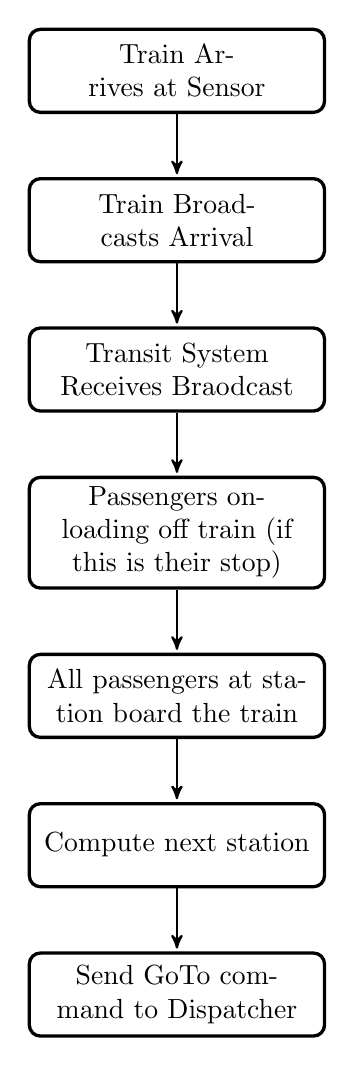
\begin{tikzpicture}[node distance=.8cm, start chain=going below,]
    \node[chain, join] (arrival) {Train Arrives at Sensor};
    \node[chain, join] (broadcast) {Train Broadcasts Arrival};
    \node[chain, join] (receive) {Transit System Receives Braodcast};
    \node[chain, join] (process) {Passengers on-loading off train (if this is their stop)};
    \node[chain, join] (process2) {All passengers at station board the train};
    \node[chain, join] (process3) {Compute next station};
    \node[chain, join] (send) {Send GoTo command to Dispatcher};
  \end{tikzpicture}
  \\[1\baselineskip]
\end{center}
\subsection{Station Allocation}
\\[1\baselineskip]
\subsection{Passenger System}
Each passenger in the system has their own destination.  Destinations are assigned ranedomly when a passenger is created at a station; a passenger may already be at the station of their choice, in which case they are simply done.  Each passenger has an associated weight which begins at $1$.  When determining which station a train should go to next, the system computes weights for each station as the sum of the weights of the passengers who want to go to that destination; the largest weighted station is the next station that train is routed to.  When a passenger is on a train and arrives at a station but does not get off (it is not their station), their weight increases by $1$.  This allows the system to account for situations where there would be only one passenger wanting to go to a particular station, and as a result, they would never get off because the other stations would be valued higher.  In addition, as a part of the passenger system, passengers also communicate to voice their opinions on the service to a channel that can be viewed by running the command ``intercom'' from within the \texttt{Shell}.  These get progressively billigerant the longer the passengers are on the train without reaching their destination.
\\[2\baselineskip]
\section{Known Errors}
\\[2\baselineskip]
\section{MD5}
\lstinputlisting{md5}
\end{document}
